\chapter{Pendahuluan}
Selalu ada aspek negatif dari sebuah pemanfaatan teknologi.
Teknologi informasi tidak lepas dari masalah ini.
Ada banyak manfaat dari teknologi informasi.
Sayangnya salah satu aspek negatifnya adalah masalah keamanan
({\em security}).

Banyak tulisan dan buku yang mengajarkan cara merusak sebuah
sistem informasi. Sementara itu buku yang mengajarkan cara
pengamanannya agak minim. Demikian pula, ilmu untuk mengamankan
sistem berbasis teknologi informasi juga harus lebih banyak
diajarkan.

%%%
\section{Keamanan Informasi}
Ketika kita berbicara tentang {\em security}, yang muncul dalam
benak kebanyakan orang adalah {\em network security}, keamanan jaringan.
Padahal sesungguhnya yang ingin kita amankan adalah \textbf{informasi}.
Bahwa informasi tersebut dikirimkan melalui jaringan adalah benar,
tetapi tetap yang ingin kita amankan adalah informasinya.
Nanti akan kita bahas lebih lanjut mengapa demikian.
Maka judul dari buku ini adalah ``Keamanan Informasi''.

%%%
\section{Beberapa Contoh Kasus}
Untuk menunjukkan betapa banyaknya masalah keamanan informasi,
berikut ini ada beberapa contoh kasus-kasus.
Contoh ini bukanlah daftar yang komplit, melainkan hanya sampel
dari kondisi yang ada. Bahkan, kemungkinan kondisi yang ada
lebih parah daripada contoh-contoh ini.

Beberapa contoh kasus di luar negeri (diurutkan berdasarkan
tahun kejadiannya) antara lain dapat dilihat dari daftar berikut.

\begin{enumerate}
\item 2006-2008. Tahun-tahun ini ditandai dengan mulai masuknya
   aspek manajemen ke dalam bidang keamanan informasi.
   Standar ISO (mulai dari 17799 dan kemudian menjadi seri 27000)
   mulai digunakan di berbagai instansi.
   Adanya bencana alam (tsunami, banjir, gempa, dan sejenisnya)
   membuat orang mulai memikirkan keberlangsungannya sistem IT.
   Perangkat IT semakin mengecil dalam ukuran sehingga mulai dibawa
   pengguna ke kantor. Misalnya pengguna membawa sendiri akses
   internet dengan menggunakan handphone 3G.
   Penggunaan kartu sebagai pengganti uang juga mulai populer.
   (Less cash society.)

\item 2013. Virus masih tetap mendominasi masalah.
   Pencurian identitas ({\em identity theft}) mulai marak.
   Cyber war mulai menjadi bagian dari diskusi.
\item 2014. Heartbleed dan Bash Bug.
   (Yang ini lebih mudah dijelaskan dengan menggunakan gambar.
   Sayangnya saya tidak memiliki hak untuk memasukkan gambar tersebut
   ke dalam buku ini. Di kesempatan berikutnya akan saya usahakan
   memberi penjelasan dengan kata-kata dulu.)
\item 2014. Bursa Singapura terganggu karena masalah software.
   Perdagangan saham sempat terhenti.
\item 2016.
   Sebuah firma hukum di Panama bernama Mossack Fonseca (MF)
   mengalami kebocoran data.
   Data yang bocor berupa tabungan / investasi orang-orang terkenal
   dari beberapa negara (termasuk Indonesia).
   Kasus ini disebut {\em Panama Papers Breach}.
   Kebocoran ini diduga karena {\em Slider plugin} yang digunakan
   oleh situsnya (yang menggunakan Wordpress) sudah kadaluawarsa dan
   memiliki kerentanan. Hasil eksploitasi memperkenankan orang untuk
   mengambil berkas sesukanya.
\item 2016. 
   CCTV digunakan sebagai bagian dari Distributed DoS attack.
   Ini menunjukkan bahwa perangkat yang menjadi bagian dari
   Internet of Things (IoT) dapat menjadi target serangan
   untuk kemudian dijadikan ``anak buah'' (zombie) untuk
   menyerang tempat lain.
   Kode sumber Mirai yang digunakan untuk melakukan penyerangan
   tersedia di internet. Jika kita tidak siap, ini dapat menjadi
   masalah yang berikutnya.
\item 2016.
   Serangan DDoS terhadap berbagai DNS (Domain Name System) servers.
   Serangan menggunakan bantuan {\em botnet}
   sehingga menghabiskan {\em bandiwdth} jaringan dalam orde
   Gbps.
\item 2017.
   Sebuah kampus di Amerika Serika mengalami masalah di jaringan internalnya.
      Ternyata ada banyak paket dari segmen mesin minuman (atau segmen IoT).
      Perangkat IoT ternyata diretas (melalui coba-coba password secara
      brute-force). Kemudian perangkat tersebut menyerang DNS dari kampus.
\item Februari 2017. 
   Layanan cloud dari Amazon.com berhenti berfungsi (down) selama beberapa jam.
      Berbagai perusahaan yang menyediakan layanan untuk publik dan kebetulan
      menggunakan layanan cloud (S3) dari Amazon ikut berhenti. Setelah
      diteliti, penyebabnya adalah salah ketik (typo) dari salah seorang
      operator~\footnote{Catatan dari Amazon dapat dibaca di sini: https://aws.amazon.com/message/41926/}.
   \item Mei 2017. Dunia digemparkan dengan Ransomware WannaCry yang menyerang
      hampir semua versi dari sistem operasi Microsoft Windows. Penyerangan
      memanfaatkan kelemahan dari SMBv1. Sebetulnya dari sisi teknis,
      ransomware ini tidak lebih hebat dari yang lain-lainnya tetapi nampaknya
      wawasan akan keamanan mulai terbangun. (Meskipun ada reaksi yang terlalu
      berlebihan.) Salah satu dokumentasi cara penanganannya dapat dibaca di
      blog~\cite{brwannacry}\footnote{https://rahard.wordpress.com/2017/05/14/
      penanganan-ransomware-wannacry/}.
\item 27 Mei 2017. Sistem komputer dari penerbangan British Airways (BA) gagal
   berfungsi. Akibatnya seluruh penerbangan terkait dengan BA dihentikan.
      Penumpang terkatung-katung. Diberitakan bahwa software tidak berfungsi
      dan kemungkinan penyebabnya adalah masalah {\em power}.
   \item Juni 2017. Kembali terjadi serangan ransomware yang diberi nama Petya.
      (Nama ini diberikan karena pada awalnya diduga kodenya mirip dengan kode
      yang diberi nama Petya, tetapi penelusuran lebih jauh ternyata
      menunjukkan bahwa kodenya berbeda.) Pada dasarnya ransomware ini
      melakukan eksploitasi kelemahan pada SBM v1, seperti pada ransomware
      WannaCry. Diduga eksploit ini juga berasal dari eksploit EtherBlue yang
      dikembangkan oleh NSA. Ransomware Petya ini pertama kali ditemukan di
      Ukraina. Diperkirakan awalnya disebarkan melalui software akunting yang
      harus digunakan oleh perusahaan yang memiliki kontrak dengan pemerintah
      Ukrainia. Itulah sebabnya ada dugaan lain bahwa sebetulnya serangan ini
      ditargetkan untuk menyerang atau mengacaukan Ukraina. Penyebaran
      ransomware ini agak terbatas karena mekanisme penyebarannya melalui
      jaringan lokal, bukan internet meskipun upaya penyebaran melalui 
      {\em pishing} juga ada..
   \item 13 September 2017. Aplikasi chat Telegram down sehingga tidak dapat
      digunakan. Diduga permasalahan disebabkan oleh listrik di data center
      mereka yang berada di Singapura. Ini adalah masalah {\em availability}.
      Padahal permasalahan listrik di data center Singapura seharusnya tidak
      menjadi masalah.
      \begin{figure}[ht]
      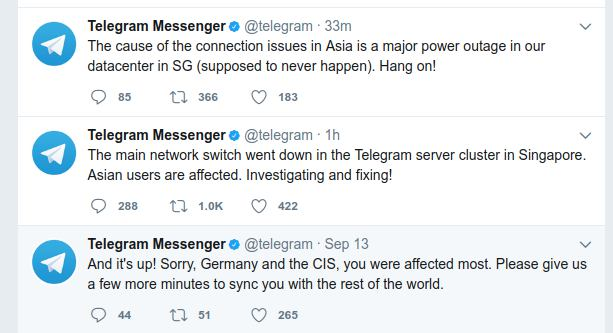
\includegraphics[width=1.0\linewidth]{graphics/telegram-down.jpg}
      \caption{Telegram down}                                                   
      \label{fig:telegram-down}                                                 
      \end{figure}
\end{enumerate}

Selain contoh-contoh di atas, tentunya masih banyak kasus-kasus lain.
Ada yang menganalogikan ini sebagai puncak dari {\em iceberg}.
Di bawah laut lebih banyak lagi masalah yang tidak terlihat.

Beberapa contoh kasus yang terkait dengan Indonesia dapat
dilihat dari daftar berikut.

\begin{enumerate}
\item 1999. Nama domain Timor Timur (.TP) diacak-acak.
   Diduga pelakunya adalah pemerintah Indonesia.
   Investigasi lebih lanjut menunjukkan bahwa ini tidak dilakukan
   oleh pemerintah Indonesia tetapi oleh seseorang (atau sekelompok)
   yang berada di Amerika Serikat.
\item 2011. Perusahaan Research in Motion (RIM) yang memproduksi
   {\em Blackberry} dipaksa untuk memiliki server di Indonesia.
   Alasan utama adalah agar dapat dilakukan {\em lawful interception},
   yaitu penyadapan secara legal untuk kasus-kasus tertentu.
   Pihak RIM keberatan. Tidak ada server RIM di Indonesia.
\item 2015. Serangan man-in-the-browser (MITB) dilakukan terhadap
   berbagai layanan internet banking di Indonesia sehingga mengakibatkan
   hilangnya uang nasabah\footnote{http://regional.kompas.com/read/
   2015/08/11/12185971/
   Kronologi. Hilangnya. Uang. Nasabah. Bank. Mandiri.
   Versi. Korban}
\item 2016. Aplikasi Pokemon Go mulai muncul dan ramai digunakan.
   Aplikasi ini menggunakan lokasi pengguna sebagai bagian dari
   permainannya, yaitu untuk menampilkan monster Pokemon sesuai
   dengan lokasi.
   Selain itu, foto dari lingkungan sekitarnya dapat juga kita ambil
   dan kita bagikan (share) dengan orang lain melalui media sosial.
   Aplikasi ini dilarang digunakan di lingkungan milter dan
   pemerintahan karena dikhawatirkan dapat membocorkan data rahasia.
   (Sebetulnya ada banyak aplikasi lain yang juga menggunakan data
   lokasi seperti {\em Waze} dan {\em Google Maps}, tetapi ini tidak
   ``terlihat''. Bahkan lebih berbahaya lagi adalah penggunaan
   layanan email gratisan untuk akun resmi pemerintahan atau instansi
   lain di Indonesia.)
\item 2016.
   Berbagai {\em market place} (seperti Tokopedia, Bukalapak, dll.)
   dan aplikasi handphone (seperti Go-Jek) diserang oleh orang
   yang mencoba melakukan password cracking.
   Asumsinya adalah seseorang akan menggunakan userid (alamat email)
   dan password yang sama untuk situs-situs tersebut.
   Identitas yang bocor di sebuah layanan (web site, application)
   dicoba digunakan di tempat lain. 
\item 2016. Topik pembentukan ``Badan Cyber Nasional (BCN)''
   mulai hangat dibicarakan.
\item 2017. Seorang (beberapa?) mahasiswa di sebuah perguruan tinggi
   di Indonesia meminta bantuan cracker untuk mengubah nilainya di
   sistem informasi kampusnya.
\item Maret 2017. Listrik dari tempat data center dari sebuah ISP mati sehingga
   layanannya terhenti. Beberapa {\em electronic market places} ikut terkena
      imbasnya karena menggunakan layanan ISP tersebut.
\item Agustus 2017. Satelit Telkom 1 mengalami masalah sehingga ribuan ATM
   dari berbagai bank di Indonesia tidak dapat beroperasi. Satelit ini
   memang sudah habis masa operasinya, meskipun diperkirakan masih dapat
   digunakan beberapa tahun lagi. Dipertanyakan kesiapan dari {\em business
   continuity planing} dari layanan ATM bank.
\end{enumerate}

Saat ini semakin banyak lagi masalah keamanan yang ditemui.
Hal ini disebabkan semakin banyak pemanfaatan teknologi informasi dan
jaringan internet.
Selain itu teknik untuk menemukan lubang keamanan juga semakin
canggih sehingga lebih banyak ditemukan kelemahan-kelemahan tersebut.

Sebuah survey yang dilakukan oleh {\em Information Week} di Amerika
Serikat (tahun?) menunjukkan bahwa hanya 22 persen manager yang
menganggap keamanan sistem informasi sebagai hal yang penting.
Bagaimana meyakinkan mereka untuk melakukan investasi di pengamanan?

Rendahnya kesadaran atas masalah keamanan (lack of security awareness)
merupakan salah satu kunci utama munculnya masalah keamanan.
Para praktisi juga masih menjalankan kebiasaan buruk,
seperti misalnya berbagi password admin.

Masalah keamanan informasi yang biasanya berupada data teknis
harus diterjemahkan ke angka finansial agar dapat dimengerti 
oleh pihak pimpinan.
Sebagai contoh, di Inggris ada survey mengenai berapa biaya
yang dikeluarkan perusahaan jika sistem mereka tidak dapat
diakses ({\em down}).



\section{Security Life Cycle}
Banyak orang yang beranggapan bahwa masalah keamanan informasi
dapat dipecahkan dengan membeli produk keamanan,
misalnya firewall, anti-virus, dan seterusnya.
Kemanan informasi sebetulnya berupa sebuah siklus
sebagaimana ditampilkan pada Gambar~\ref{fig:security-life-cycle}.

\begin{figure}[ht]
\fbox{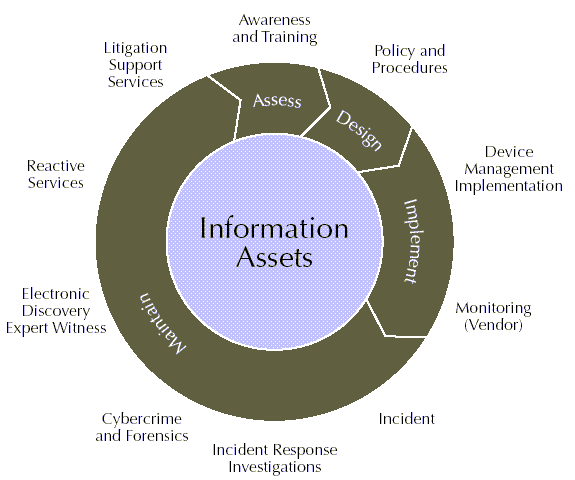
\includegraphics[width=1.0\linewidth]{graphics/security-life-cycle.png}}
\caption{Security Life Cycle}
\label{fig:security-life-cycle}
\end{figure}

Sesuatu yang akan kita amankan disebut dengan ``aset''. Untuk itu, langkah
pertaman dalam pengamanan adalah menentukan aset yang ingin dilindungi. Apa saja
yang dianggap sebagai aset harus ditentukan bersama dengan pemilik dari sistem
(aplikasi, data, dsb.) sebab mereka yang mengetahui mana aset dan mana yang
bukan aset.
Proses ini disebut {\em assesment} dan dapat dilakukan dengan melalui training
atau {\em awareness} terhadap pihak-pihak terkait. Seringkali pemilik aplikasi
memahami mana asetnya tetapi pihak operasional (orang-orang IT yang diberi
tugas untuk mengamankan sistem) tidak tahu.

Setelah mengetahui aset yang ingin diamankan, aset tersebut harus kita beri
harga (value). Pengamanan nantinya akan disesuai dengan dengan nilai dari aset
tersebut. Akan sulit kita melakukan investasi pengamanan yang biasanya lebih
mahal dari nilai asetnya. Sebagai contoh, jika kita memiliki sebuah komputer
yang harganya Rp.~5.000.000,- maka akan sulit untuk menerima biaya pengamanan
yang harganya Rp.~100.000.000,- (lebih mahal). Biaya pengamanan harus lebih
murah daripada nilai asetnya. Jika biaya pengamanan lebih mahal, mungkin lebih
baik membeli barang sejenis saja sebagai duplikat.

Untuk hal-hal yang terkait dengan teknologi informasi, pendaftaran aset-aset
ini tidak mudah karena ada hal-hal yang tidak terlihat secara kasat mata.  Aset
ini dapat kita bagi menjadi tiga (3) jenis; {\em hardware}, {\em software}, dan
data. Mari kita mulai mencoba mendata.

Aset yang berbentuk perangkat keras (hardware) agak ``mudah'' didata karena
terlihat oleh mata, tetapi ada beberapa hal yang membuatnya menjadi susah.
Salah satunya adalah nilai dari aset tersebut. Harga komputer cenderung jatuh
dengan cepat. Berapa depresiasi dari sebuah server?  Contoh-contoh aset
perangkat keras antara lain komputer, router, perangkat jaringan, disk, dan
seterusnya. Apakah notebook termasuk aset atau barang habis? Bagaimana dengan
USB flashdisk? Apakah itu termasuk aset juga?

Beberapa kejadian terkait dengan kesulitan mendata perangkat keras antara lain
tidak diketahuinya pemilik dari perangkat tersebut. Database perangkat keras
sering tidak tersedia. Sebagai contoh, sering kali tidak diketahui harddisk dan
lokasi server yang menggunakan disk tersebut.

Jika pendataan perangkat keras sudah susah, maka pendataan perangkat lunak
lebih susah lagi. Masalahnya, perangkat lunak tidak terlihat secara kasat mata
sehingga pendataannya harus melalui pemilik layanan / pemilik aplikasi. Sebagai
contoh, sebuah layanan online memiliki aplikasi di server web dan juga database
di server database. Aplikasi-aplikasi tersebut berbentuk beberapa perangkat
lunak yang tentunya memiliki harga.

Penentuan harga (nilai) dari perangkat lunak cukup rumit. Untuk aplikasi yang
dibeli, dapat digunakan harga pembelian tersebut. Bagaimana menentukan harga
aplikasi yang dikembangkan sendiri? Ada yang menggunakan jumlah waktu
pengembang (dalam {\em man days}) yang kemudian dikalikan dengan honor (gaji)
orang tersebut. Itulah harga dari aplikasi tersebut. Lantas bagaimana dengan
produk {\em free software} atau (sebagian dari) {\em open source} yang
kebanyakan dapat diperoleh secara gratis? Bagaimana menentukan harga mereka?
Ini masih menjadi pertanyaan. Hal lain yang menyulitkan adalah berapa
depresiasi dari perangkat lunak?

Bagian selanjutnya dari aset teknologi informasi adalah data. Jika pendaftaran
aset hardware dan software sudah sukar, pendaftaran data lebih sukar lagi. Data
apa saja yang dimiliki oleh sistem? Pada umumnya data apa saja yang tersedia
tidak terdaftar. Masing-masing aplikasi hanya memiliki data tersendiri.

Penentuan harga dari data lebih sukar lagi. Sebagai contoh, berapa harga data
transkrip mahasiswa? Bagi mahasiswa, data tersebut sangat berharga sehingga
harus dilindungi. Bagi orang lain, data tersebut mungkin tidak ada nilainya.
Maukah Anda membeli data transkrip mahasiswa ITB seharga Rp.~30.000.000,-~?
Saya yakin tidak ada yang mau. Bagaimana jika Rp.~3.000.000,- saja? Mungkin
masih tidak. Bagaimana jika Rp.~3.000,-~? Mungkin mau. Apakah nilai dari data
transkrip tersebut hanya tiga ribu rupiah? Jika iya, bagaimana nilai
perlindungan yang akan kita berikan?


Setelah mengetahui aset yang akan dilindungi, langkah pertama yang dilakukan
adalah melakukan desain pengamanan. Hal ini dilakukan dengan mengembangkan
kebijakan dan prosedur ({\em policies and procedures}). Banyak yang melupakan
langkah ini dan langsung melakukan implementasi, tetapi tanpa PnP ini akan
sulit. Sebagai contoh, siapa yang boleh melakukan akses kepada data transkrip
tersebut? Ini dituangkan dalam kebijakan. Tanpa kebijakan ini, perangkat
pengamanan yang ada (authorization dan access control) akan sulit diterapkan.
Rules apa yang akan dipakai? Banyak kejadian sistem pengamanan diterapkan
dengan salah karena tidak memiliki desain yang benar.

Desain pengamanan ini kemudian diterapkan secara teknis melalui perangkat
pengamanan ({\em security devices}). Penerapan ini dapat meminta bantuan
vendor. 

Meskipun sudah diterapkan pengamanan, insiden keamanan akan tetap dapat
terjadi. Ketika insiden ini terjadi, maka harus dilakukan investigasi terlebih
dahulu. Apakah insiden yang terjadi tersebut benar-benar insiden ataukah
kejadian biasa saja? Jika memang itu adalah insiden, maka akan diproses lebih
lanjut sesuai dengan kebijakan dan prosedur yang ada.

Ini kemudian menjadi siklus; {\em security life cycle}. Banyak orang yang masih
menganggap {\em security} adalah sebuah produk sehingga mereka lebih fokus
kepada pembelian produk pengamanan tertentu tanpa memperhatikan faktor lain
(misalnya aset mana yang akan dilindungi). Ini seperti mengatasi sakit kepala
dengan menggunakan obat penghilang rasa sakit tanpa perlu mencari tahu apa
sumber permasalahan sesungguhnya.


\section{Keamanan Dari Berbagai Elemen Sistem}
Dahulu, ketika kita berbicara tentang {\em security}, maka yang ada dalam
kepala sebagian besar orang adalah {\em network security} (keamanan jaringan
komputer). Padahal sistem teknologi informasi tidak hanya jaringan saja. Ada
elemen-elemen lain di sistem.

Sebuah sistem berbasis teknologi informasi memiliki beberapa elemen (komponen),
yaitu komputer (host, server, workstation), jaringan (beserta perangkatnya),
dan aplikasi (software, database). Keamanan dari masing-masing elemen tersebut
akan berbeda penanganannya.

\subsection{Computer Security}
{\em Computer security} (keamanan komputer) terkait dengan keamanan komputer,
yang boleh jadi merupakan server, workstation, notebook, dan sejenisnya.
Seringkali ini disebut juga sebagai {\em host security}.

Permasalahan yang muncul pada keamanan komputer terkait dengan sistem operasi
yang digunakan, {\em patch} yang sudah dipasang, konfigurasi yang digunakan,
serta keberadaan aplikasi yang ada. Seringkali sistem operasi yang digunakan
sudah kadaluwarsa dan sudah ditemukan beberapa kerentanan (vulnerability) pada
sistem operasinya.

\subsection{Network Security}
Saat ini sebagian besar sistem terhubung dengan jaringan (apapun jenis
jaringannya). Ada beberapa masalah terkait dengan keamanan jaringan, seperti
misalnya penyadapan data, modifikasi data, dan juga serangan {\em Denial of
Service} terhadap jaringan dengan membanjiri jaringan dengan paket yang sangat
banyak (sangat besar).


\subsection{Application Security}
Boleh jadi komputer (server) yang digunakan sudah aman dan jaringan yang
digunakan sudah aman, tetapi aplikasi (software) yang digunakan memiliki
kerentanan sehingga data dapat diambil (atau diubah) oleh orang yang tidak
berhak. Contoh yang sering terjadi saat ini adalah {\em SQL injection}.

Terkait dengan application security adalah keamanan sistem database.
Ternyata penanganan masalah keamanan database mirip dengan penanganan keamanan
jaringan (bukan aplikasi).

Topik keamanan aplikasi atau software mulai menjadi penting dan ini menjadi
topik buku tersendiri.
